\section{Tiny Tapeout 3}
\label{sec:tinytapeout3}

Tiny Tapeout 3 opened in March 2023 and \qty{100} new designs were submitted by participants. To fill the remaining space an additional \qty{149} designs were added from TT01.

For Tiny Tapeout 3 the two clock buffers of Tiny Tapeout 1 and 2 were replaced by an inverting clock buffer design, with only one buffer between the clock input and output. Fig. ~\ref{fig:TT02_vs_TT03} shows a comparison between the TT02 and TT03 clock buffer designs. By inverting the clock between each design any asymmetry in the clock pulse is evenly spread across the negative and positive cycles.

\begin{figure}[!t]
\centering
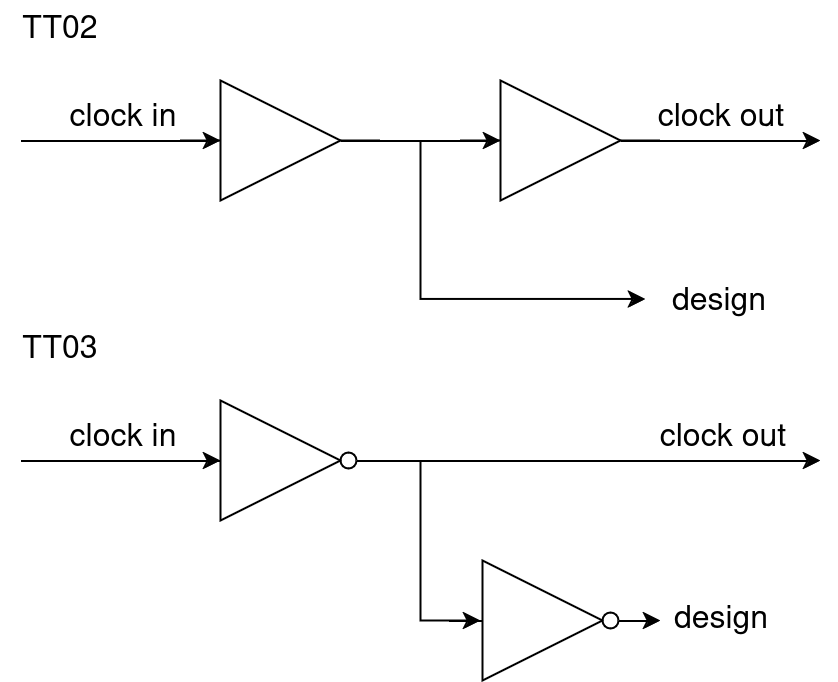
\includegraphics[width=\columnwidth]{./Figs/tt02 vs tt03 scanchain clock.png}
\caption{The Tiny Tapeout 3 architecture buffers the output from the clock network into each design. Clock polarity is alternated between designs to minimize asymmetry between positive and negative cycles.}
\label{fig:TT02_vs_TT03}
\end{figure}

Silicon was received in January 2024, and at the time of writing was being assembled for delivery to customers by March 2024.

Following the closure of Tiny Tapeout 3 an invitational experimental shuttle dubbed Tiny Tapeout 3.5 ~\cite{tinytapeout03p5} was submitted for production. This featured \qty{32} designs, each testing and previewing some of the changes planned for Tiny Tapeout 4 as detailed in the next section. Two of these designs included a power gate, as a stepping stone to supporting analog and mixed signal designs.

The finished design was submitted for production on Efabless chipIgnite 2306C.
Silicon was received in December 2023 and at the time of writing was being assembled for testing.
